\documentclass[12pt]{report}			% Začátek dokumentu
\usepackage{MP}							% Import stylu

\author{Jakub Skalka}
\title{Algologický průzkum vodních ploch v lokalitě Lipí}
\date{Někdy 2024}
\vedouci{}
\place{V Českých Budějovicích}
\skolnirok{2024/2025}
\logo{
\includegraphics[scale=1.25]{GJ8_logotyp}}

\begin{document}
\pagenumbering{roman}                   % číslování stránek římskými číslicemi
	\mytitlepage						% Vygenerování titulní strany
	
	\prohlaseni{
		Prohlašuji, že jsem tuto práci vypracoval samostatně s vyznačením všech použitých pramenů.
	}	
	
	\abstrakt{
		\lipsum[1]						% Abstrakt
	}{
		\lipsum[1]						% Klíčová slova
	}
	
	\podekovani{
		Tímto chci poděkovat všem, kteří mi pomohli s touto prací. Hlavně 
	}
	
   {\tableofcontents\newpage}			% Obsah
	
\addtocounter{page}{1}		% Posunutí countru stránek
\pagenumbering{arabic}		% Číslování stránke arabskými číslicemi
	\chapter*{Úvod}
	
		\lipsum[1]	
	
	
	\part{Teoretická část}
	
		\chapter{Název úvodní kapitoly}
			
			\section{O-notace}
				Odkaz v závorkách: \parencite[see][page 900]{einstein}\\
				Odkaz: \cite{knuthwebsite}\\
				A odkaz pod čarou: \footcite[see][s. 42]{latexcompanion}\\
				Dobrý den, ahoj, \gls{atd}\\
				Praha, \gls{tj} hlavní město ČR
				
				\begin{table}
				  \caption{Testovací tabulka}
				  \label{tab:test2}
				  \begin{tabular}{ccccc}
                  1 & 1 & 1  & 1  & 1  \\
                  1 & 2 & 3  & 4  & 5  \\
                  1 & 3 & 6  & 10 & 15 \\
				  1 & 4 & 10 & 30 & 45
				  \end{tabular}
				\end{table}

				\lipsum[2]

			\section[X-krát Abeceda]{Abeceda Abeceda Abeceda Abeceda Abeceda Abeceda Abeceda Abeceda Abeceda Abeceda }
			%%% v obsahu se objeví jen to co je v hranatých závorkách
				\begin{figure}
				  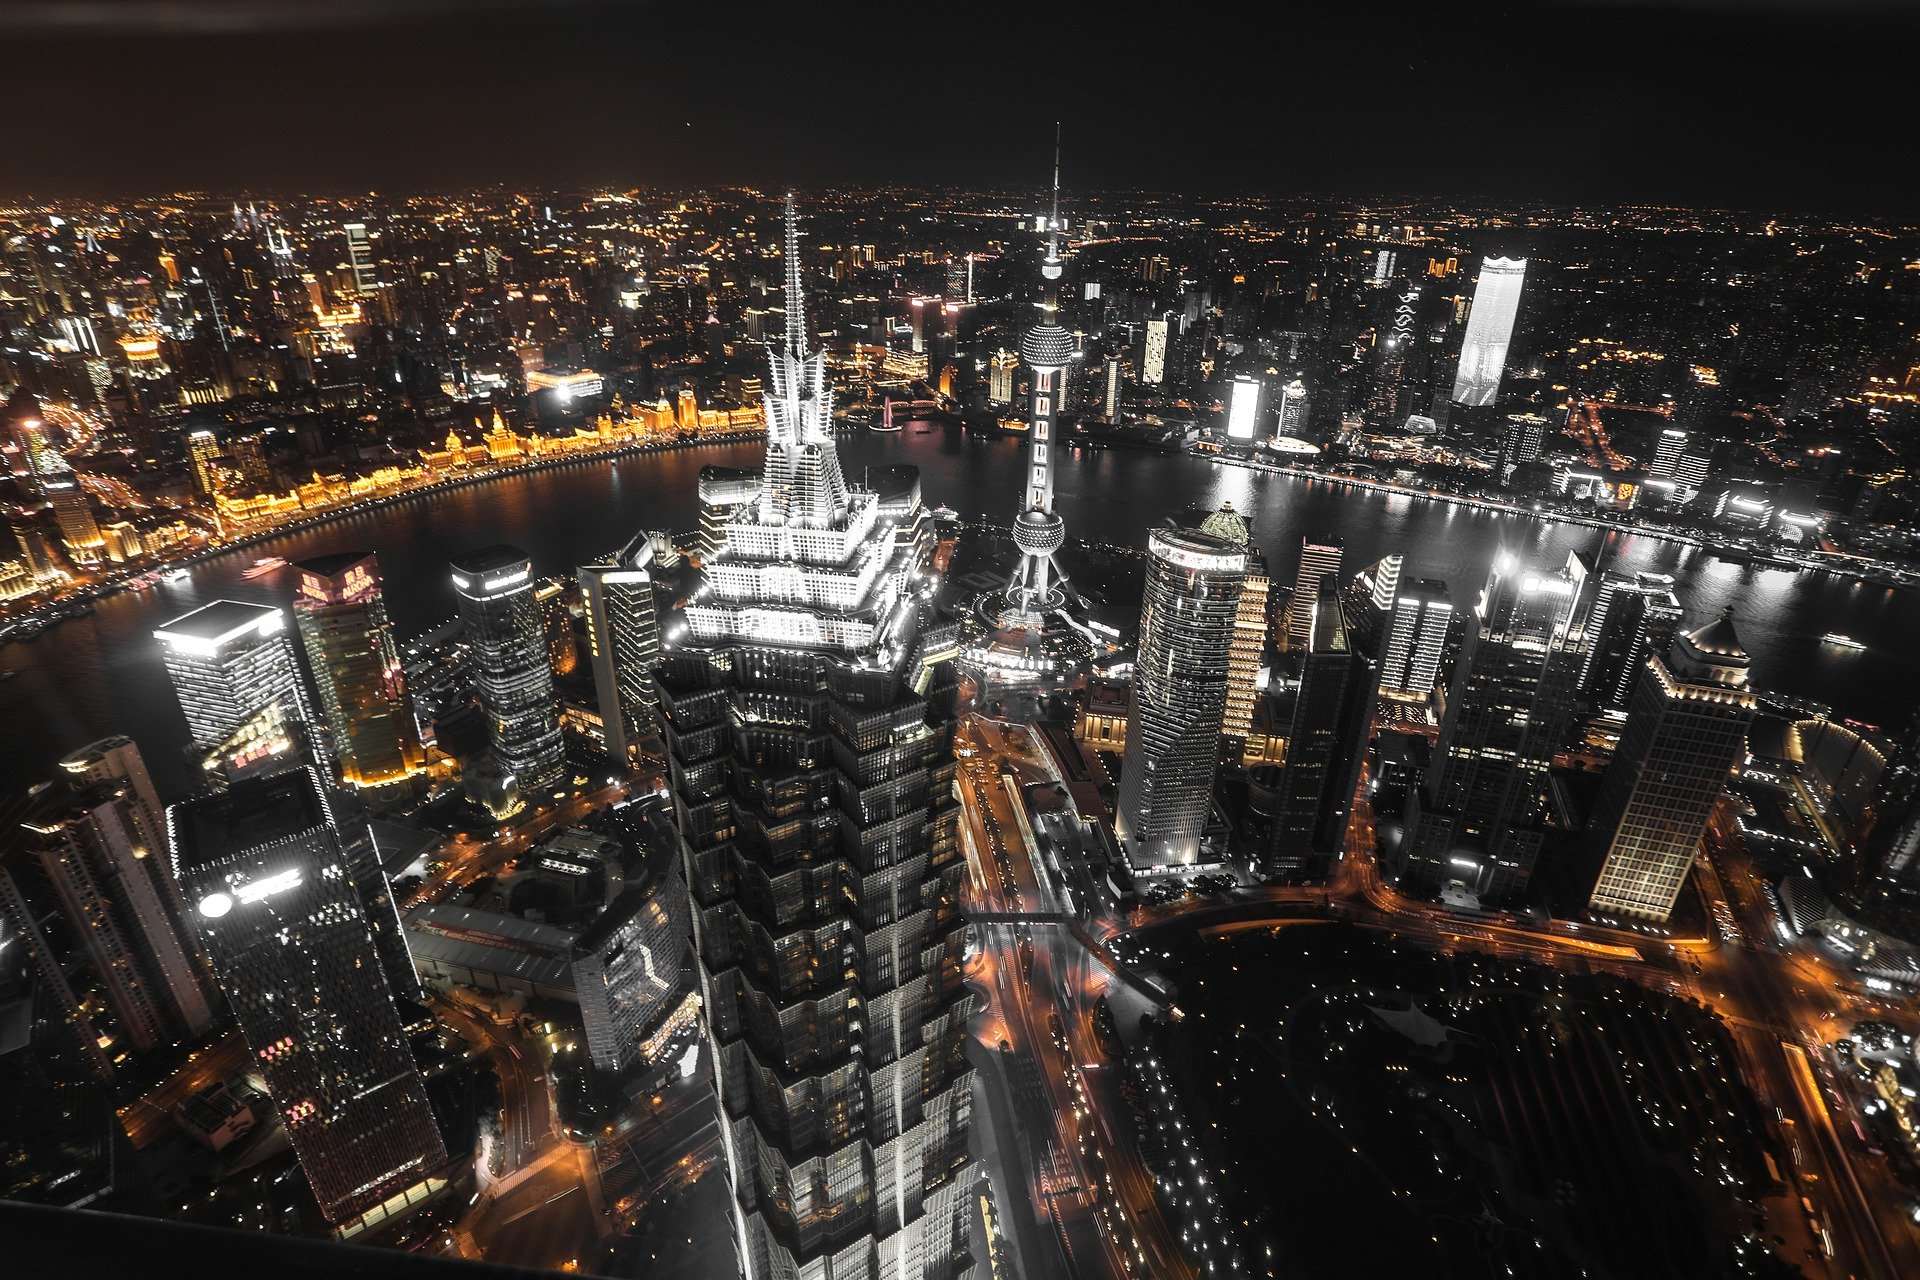
\includegraphics[width=\linewidth]{test.jpg}
				  \caption{Testovací}
				  \label{fig:test}
				\end{figure}
				Obrázek \ref{fig:test} ukazuje Shangai z Pixabay.\\
				Tabulka \ref{tab:test2} ukazuje hádejte, co.
		
	\lipsum[3]

	\part{Praktická část}

\section{Výpisy použitých programů}

\lipsum[1]	

Výpis programu \nameref{lst:hello_world}  naleznete ve výpise \ref{lst:hello_world}.

\begin{lstlisting}[title={Program hello.c}, caption={hello.c}, label={lst:hello_world}]
#include <stdio.h>
#define CISLO 10

int main(void) {
	int i = CISLO;

	print("Hello World!\n");
	print("%d", i);

	return (0);
}
\end{lstlisting}

\lipsum[1]	

\begin{lstlisting}[numbers=none, title={Příklad výstupního souboru}]
11.0524
5.5954
6.7996
13.8584
15.1357
Soucet: 52.4415
\end{lstlisting}

	\chapter*{Závěr}
	
		\lipsum[1]
	
	\nocite{*}
    \printbibliography					% Vytvoří seznam literatury
	\addcontentsline{toc}{chapter}{Bibliografie}
    \printglossary[title={Zkratky}]		% Vytvoří seznam zkratek
    \listoffigures						% Vytvoří seznam obrázků
    \listoftables						% Vytvoří seznam tabulek

    \begin{appendices}
	\chapter{Fotky z pokusů}	
	\lipsum[1]
    	%\pitem{Fotky z pokusů}
    	%\eitem{Vlastní program}
    	%\eitem{Dokumentace}
    	%\eitem{Testovací data}
	\chapter{Příloha další }
	\end{appendices}
\end{document}
